\section{Conception}

This section will detail the conception and the class diagram of our project. The following graph shows the different classes we used in the project.

\begin{figure}
 \centering
 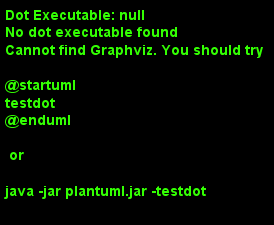
\includegraphics{../uml/classDiagram.pdf}
 \caption{Class diagram}
\end{figure}

\subsection{StaticGesture and StaticGestures}

StaticGesture (without s) is not really a class, it is an enum that holds all of the static gesture that are possible to detect. The main role of using an enum is not to have to handle the value of each gesture and make it more user friendly. It also simplify the use within the functions for the developper.

StaticGestures (with an s) is the class which allow the user to detect the StaticGesture within a frame. To make it lighter a simple set of hand (Leap::HandList) is required when the object is created. A new object is required to be created each time a new HandList is used. This last part is one of the possible improvement on the code (even if the creation of the new object make sense and is viable).

\subsection{GestValidator}

As far as StaticGestures is concerned, a new gesture is possibly detected after each new frame. Since this is not usable for the user, the class GestValidator was added. This class allows to set a number of frame on which the the gesture needs to be in order to be validated.
Within this class, two functions need to be detailed, update and SetGesture. Their aim can seem identical when they are not, update allows the user to update the gesture within the GestValidator object i.e 11th gesture is CLOSED\_HAND whereas setGesture set the gesture count to 0 i.e 1st gesture is now CLOSE\_HAND (and if update is used after that we have 2nd gesture is ...).

\subsection{DetectionListener}

This class is one of the simplest one, it is one of the class given within the LeapMotion api, it allows the user to define what will happen when a certain event is triggered.
Here we use it to handle the mode selection (one or two). And to update the detection of the gesture.

\subsection{ModeHandler}

This is the class used to handle the different mode which are available within our program (1 and 2). The user only need to call to the function modeX to handle the required mode. The class will handle the communication with the robot through the Communicator (see below). Each previous state is stored and this class should not be re-instansciated after each new frame.

It is within this class that the filter is used (mode 2) in order to smoothen the output when communicating with the robot.

\subsection{Communicator}

This is thee class that handle the TCP communication. It is a simple class which will connect to the robot and then send the data through the function sendData(). This last function allows the user to set a delay or not in order to give the robot some times to carry out the action that is required.
